\documentclass[12pt]{article}

\usepackage{graphicx}
\usepackage{paralist}
\usepackage{amsfonts}
\usepackage{amsmath}
\usepackage{hhline}
\usepackage{booktabs}
\usepackage{multirow}
\usepackage{multicol}
\usepackage{url}

\oddsidemargin -10mm
\evensidemargin -10mm
\textwidth 160mm
\textheight 200mm
\renewcommand\baselinestretch{1.0}

\pagestyle {plain}
\pagenumbering{arabic}

\newcounter{stepnum}

%% Comments

\usepackage{color}

\newif\ifcomments\commentstrue

\ifcomments
\newcommand{\authornote}[3]{\textcolor{#1}{[#3 ---#2]}}
\newcommand{\todo}[1]{\textcolor{red}{[TODO: #1]}}
\else
\newcommand{\authornote}[3]{}
\newcommand{\todo}[1]{}
\fi

\newcommand{\wss}[1]{\authornote{blue}{SS}{#1}}

\title{Assignment 4, Design Specification}
\author{COMP SCI 2ME3}

\begin{document}

\maketitle

This Module Interface Specificaiton (MIS) document contains the modules,
types, and methods for implementing the game 2048. At the start of each
game, 2 numbers are created in a random location on a 4x4 grid. The number
created has 90\% chance of being a 2, and a 10\% chance of being a 4. The
user must combine matching numbers together to eventually create the number
2048 in order to win. The numbers on the board can be shifted in the
desired direction using the arrow keys, and if there is any matching
numbers present in the direction being shifted, the numbers will combine.
When shifting numbers, all numbers are shifted in the input direction as
far as possible. For combining numbers, a number can only combine once for
a given movement. For example, shifting [2,2,2,2] to the right will not
from [\_,\_,\_,8], but [\_,\_,4,4]. Which can be then shifted right one
more time to form [\_,\_,\_,8]. On the gameboard, the Row numbers increase
top to bottom, and column number increases left to right. The game requires
a GUI to be played, and can be launched by running \texttt{Demo.java} in
the desired IDE.

\begin{center}
  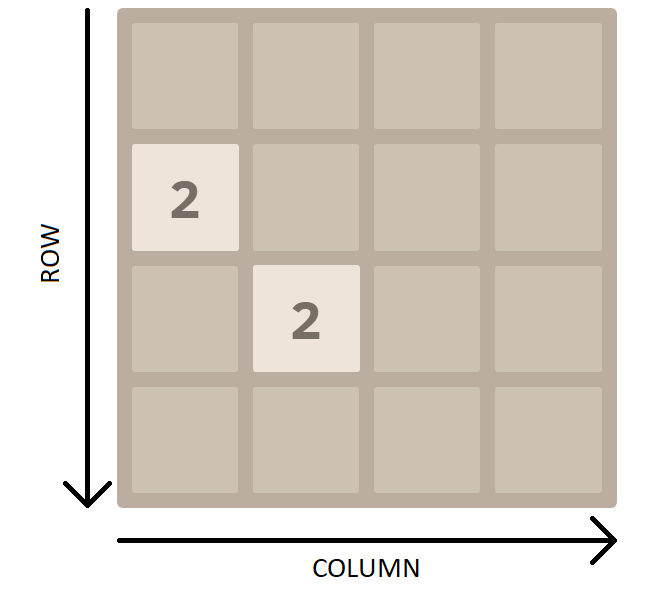
\includegraphics[width=0.7\textwidth]{naming.png}

  The above board visualization is from https://www.play2048.co/
\end{center}

\newpage

\section{Overview of the design}

This design applies the Model View design pattern. The Model View design
pattern components are \textit{GameBoard} (model Module) and \textit{Game}
(view and controller Module).


\medskip
The Module View design pattern is implemented in the following way: the
\textit{GameBoard} module stores the state of the game board and the status
of the game. As well as the main methods required for checking for win/lose
conditions and adding/movement of the board. The \textit{Game} module is
responsible for the main UI and the inputs to the game. It displays the
game board and decides the actions that should be taken on a certain key press. 

\newpage

\subsection*{Likely Changes my design considers:}

\begin{itemize}
  \item Change in UI Design (such as tile color).
  \item Addition of key inputs (such as w,a,s,d).
\end{itemize}

\newpage

\section*{Game Board Module}

\subsection*{Template Module}

GameBoard 

\subsection*{Uses}

N/A

\subsection* {Syntax}

\subsubsection* {Exported Constants}

None

\subsubsection* {Exported Types}

GameBoard = ?

\medskip

\subsubsection* {Exported Access Programs}

\begin{tabular}{| l | l | l | l | l |}
    \hline
    \textbf{Routine name} & \textbf{In} & \textbf{Out} & \textbf{Notes} &\textbf{Exceptions}\\
    \hline
    new GameBoard & & GameBoard &  &\\
    \hline
    new GameBoard & seq [4] of (seq [4] of $\mathbb{N}$) & GameBoard & For
    testing purposes &\\
    \hline
    addNewNum & & & &\\
    \hline
    addNewNum & $\mathbb{N}, \mathbb{N}, \mathbb{N}$ & & For
    testing purposes &\\
    \hline
    getScore &  & $\mathbb{N}$ & &\\
    \hline
    getHighestNum &  & $\mathbb{N}$& &\\
    \hline
    getBoard &  &seq [4] of (seq [4] of $\mathbb{N}$) & &\\
    \hline
    getCount &  &$\mathbb{N}$ & &\\
    \hline
    moveUp &  & & &\\
    \hline
    moveDown &  & & &\\
    \hline
    moveLeft &  & & &\\
    \hline
    moveRight &  & & &\\
    \hline
    gameOver & & $\mathbb{B}$ & &\\
    \hline
    \end{tabular}

\subsection* {Semantics}

\subsubsection* {State Variables}

$board$: seq of [4] (seq of [4] $\mathbb{N}$) \\
$score$: $\mathbb{N}$\\
$highestNum$: $\mathbb{N}$

\subsubsection* {State Invariant}

None

\subsubsection*{Assumptions}

\begin{itemize}
    \item Arugments given to the methods created for testing purposes will be of the
    correct type.
    \item Assume there is a function $random$ that generates a random value
    between 0 and 1. 
    \item Assume final results are rounded to the nearest integer.
\end{itemize}

\subsubsection*{Access Routine Semantics}

\noindent new GameBoard():
\begin{itemize}
    \item output: out := self 
    \item transition: 
    \begin{itemize}
        \item board := $\langle$ [[0,0,0,0], [0,0,0,0], [0,0,0,0],
        [0,0,0,0]] $\rangle$\\
        \phantom{board := }$\langle random() * 9 \equiv 0 \Rightarrow
       board[i][j] := 4 | 2$ where $i = random() * 3 \land j = random() * 3
       \land \exists(board[i][j] \equiv 0)\rangle$\\
       \phantom{board := }$\langle random() * 9 \equiv 0 \Rightarrow
       board[i][j] := 4 | 2$ where $i = random() * 3 \land j = random() * 3
       \land \exists(board[i][j] \equiv 0)\rangle$\\
       // Initializes a gameboard of 0's, and adds either a 2 (90\% chance)
       or a 4(10\% chance) into a random location twice.
        \item score := 0
        \item highestNum := ($i,j : \mathbb{N} \vert i,j \in [0..3] :
        board[i][j] > highestNum \Rightarrow highestNum := board[i][j]$)
    \end{itemize}
    \item exception: none
\end{itemize}

\noindent new GameBoard($layout$):
\begin{itemize}
    \item output: out := self 
    \item transition: 
    \begin{itemize}
        \item board := $layout$
        \item score := 0
        \item highestNum := ($i : \mathbb{N} \vert i
        \in [0..3]: (j : \mathbb{N} \vert j \in [0..3]:
        board[i][j] > highestNum \Rightarrow highestNum := board[i][j])$)
    \end{itemize}
    \item exception: none
\end{itemize}

\noindent addNewNum():
\begin{itemize}
    \item transition: board := $random() * 9 \equiv 0 \Rightarrow
    board[i][j] = 4 | 2$ where $i = random() * 3 \land j = random() * 3
    \land \exists(board[i][j] \equiv 0)$\\
    // adds either a 2 (90\% chance) or a 4(10\% chance) into a random
    location that currently has a 0.
    \item exception: none
\end{itemize}

\noindent addNewNum($value, row, col$):
\begin{itemize}
    \item transition: board[$row$][$col$] := $value$
    \item exception: none
\end{itemize}

\noindent getScore():
\begin{itemize}
    \item output: out := $score$
    \item exception: none
\end{itemize}

\noindent getHighestNum():
\begin{itemize}
    \item output: out := $highestNum$
    \item exception: none
\end{itemize}

\noindent getBoard():
\begin{itemize}
    \item output: out := $board$
    \item exception: none
\end{itemize}

\noindent getCount():
\begin{itemize}
    \item output: out := $count$ where $count$ $\equiv$ ($i : \mathbb{N} \vert i
    \in [0..3]: (j : \mathbb{N} \vert j \in [0..3]: \lnot (board[i][j] = 0)
    \Rightarrow count := count + 1 \vert count) $) \\
    // Returns the number of elements on the board that are not 0.
    \item exception: none
\end{itemize}

\noindent moveUp():
\begin{itemize}
    \item transition: board := shiftUp() $\land$ combineUp()
    $\land$ shiftUp()\\
    // Shifts all the numbers up, combines matching numbers, and shifts up again.
    \item exception: none
\end{itemize}

\noindent moveDown():
\begin{itemize}
    \item transition: board := shiftDown() $\land$ combineDown()
    $\land$ shiftDown()\\
    // Shifts all the numbers down, combines matching numbers, and shifts down again.
    \item exception: none
\end{itemize}

\noindent moveLeft():
\begin{itemize}
    \item transition: board := shiftLeft() $\land$ combineLeft()
    $\land$ shiftLeft()\\
    // Shifts all the numbers left, combines matching numbers, and shifts left again.
    \item exception: none
\end{itemize}

\noindent moveRight():
\begin{itemize}
    \item transition: board := shiftRight() $\land$ combineRight()
    $\land$ shiftRight()\\
    // Shifts all the numbers right, combines matching numbers, and shifts right again.
    \item exception: none
\end{itemize}

\noindent gameOver():
\begin{itemize}
    \item output := $\lnot(getCount() = 16) \Rightarrow False \vert (\exists((row :
    \mathbb{N} \vert row \in [0..3] : col : \mathbb{N} \vert col \in
    [0..2]: board[row][col] \equiv board[row][col+1]) \land (col :
    \mathbb{N} \vert col \in [0..3] : row : \mathbb{N} \vert row \in
    [0..2]: board[row][col] \equiv board[row+1][col])) \Rightarrow False |
    True)$\\
    //returns false if getCount() is not 16. Otherwise checks every column
    to see if any adjacent numbers are matching, and then checks ever row
    ot see if any adjacent number are matching. If no adjacent matching
    number, returns true.
    \item exception: none
\end{itemize}


\subsubsection*{Local Functions}

\noindent shiftUp()
\begin{itemize}
    \item transition: ($col : \mathbb{N} \vert col
    \in [0..3]: (row : \mathbb{N} \vert row \in [1..3]:
    board[X][col] \equiv 0 \Rightarrow board[X][col] := value
    \land board[row][col] := 0)$)\\
    where $X : \mathbb{N} | X \in [row .. 0] \land value = board[row][col]$\\
    // Goes through each column and beginning from the top shifts each
    number up continuously until the number above is not a 0, end result
    being all number are shifted and compressed to the top replacing any 0's.
    \item exception: none
\end{itemize}

\noindent combineUp()
\begin{itemize}
    \item transition: ($col : \mathbb{N} \vert col
    \in [0..3]: (row : \mathbb{N} \vert row \in [1..3]: board[row-1][col]
    \equiv value \Rightarrow board[row-1][col] := value * 2 \land
    board[row][col] := 0 \land score := score + value * 2)$)\\
    where $value \equiv board[row][col]$\\
    Combine numbers that are equal and adjacent vertically and of the two
    nubmers, the number that is north on the grid is replaced with the
    result, with the number below being replaced with a 0.
    \item exception: none
\end{itemize}

\noindent shiftDown()
\begin{itemize}
    \item transition: ($col : \mathbb{N} \vert col
    \in [0..3]: (row : \mathbb{N} \vert row \in [2..0]:
    board[X][col] \equiv 0 \Rightarrow board[X][col] := value
    \land board[row][col] := 0)$)\\
    where $X : \mathbb{N} | X \in [row .. 3] \land value = board[row][col]$\\
    // Goes through each column and beginning from the bottom shifts each
    number down continuously until the number below is not a 0, end result
    being all number are shifted and compressed to the bottom replacing any 0's.
    \item exception: none
\end{itemize}

\noindent combineDown()
\begin{itemize}
    \item transition: ($col : \mathbb{N} \vert col
    \in [0..3]: (row : \mathbb{N} \vert row \in [2..0]: board[row+1][col]
    \equiv value \Rightarrow board[row+1][col] := value * 2 \land
    board[row][col] := 0  \land score := score + value * 2)$)\\
    where $value \equiv board[row][col]$\\
    Combine numbers that are equal and adjacent vertically and of the two
    nubmers, the number that is south on the grid is replaced with the
    result, with the number above being replaced with a 0.
    \item exception: none
\end{itemize}

\noindent shiftLeft()
\begin{itemize}
    \item transition: ($row : \mathbb{N} \vert row
    \in [0..3]: (col : \mathbb{N} \vert col \in [1..3]:
    board[row][Y] \equiv 0 \Rightarrow board[row][Y] := value
    \land board[row][col] := 0)$)\\
    where $Y : \mathbb{N} | Y \in [col .. 0] \land value = board[row][col]$\\
    // Goes through each row and beginning from the left shifts each number
    to the left continuously until the number to the left is not a 0, end result
    being all number are shifted and compressed to the left replacing any
    0's.
    \item exception: none
\end{itemize}

\noindent combineLeft()
\begin{itemize}
    \item transition: ($row : \mathbb{N} \vert row
    \in [0..3]: (col : \mathbb{N} \vert col \in [1..3]: board[row][col-1]
    \equiv value \Rightarrow board[row][col-1] := value * 2 \land
    board[row][col] := 0 \land score := score + value * 2)$)\\
    where $value \equiv board[row][col]$\\
    Combine numbers that are equal and adjacent horizontally and of the two
    nubmers, the number that is further left on the grid is replaced with
    the result, with the number to the right being replaced with a 0.
    \item exception: none
\end{itemize}

\noindent shiftRight()
\begin{itemize}
    \item transition: ($row : \mathbb{N} \vert row
    \in [0..3]: (col : \mathbb{N} \vert col \in [2..0]:
    board[row][Y] \equiv 0 \Rightarrow board[row][Y] := value
    \land board[row][col] := 0)$)\\
    where $Y : \mathbb{N} | Y \in [col .. 3] \land value = board[row][col]$\\
    // Goes through each row and beginning from the right shifts each number
    to the right continuously until the number to the right is not a 0, end result
    being all number are shifted and compressed to the right replacing any
    0's.
    \item exception: none
\end{itemize}

\noindent combineRight()
\begin{itemize}
    \item transition: ($row : \mathbb{N} \vert row
    \in [0..3]: (col : \mathbb{N} \vert col \in [2..0]: board[row][col+1]
    \equiv value \Rightarrow board[row][col+1] := value * 2 \land
    board[row][col] := 0 \land score := score + value * 2)$)\\
    where $value \equiv board[row][col]$\\
    Combine numbers that are equal and adjacent horizontally and of the two
    nubmers, the number that is further right on the grid is replaced with
    the result, with the number to the left being replaced with a 0.
    \item exception: none
\end{itemize}

\newpage

\section*{View and Controller Module}

\subsection*{Module inherits JPanel, KeyListener}

Game

\subsection*{Uses}

JFrame, JPanel, KeyListener

\subsection* {Syntax}

\subsubsection* {Exported Constants}

None

\subsubsection* {Exported Types}

None 

\subsubsection* {Exported Access Programs}

\begin{tabular}{| l | l | l | l |}
    \hline
    \textbf{Routine name} & \textbf{In} & \textbf{Out} &\textbf{Exceptions}\\
    \hline
    GUI & &  &\\
    \hline
    KeyPressed & KeyEvent & &\\
    \hline
    KeyReleased & KeyEvent & &\\
    \hline
    KeyTyped & KeyEvent & &\\
    \hline
    paint & Graphics& & \\
    \hline
    drawTiles & Grahpics, $\mathbb{N}, \mathbb{N}, \mathbb{N}$ & &\\
    \hline
    \end{tabular}

\subsubsection*{Access Routine Semantics}

\section*{Semantics}

\subsubsection*{Envrionment Variables}

window: A portion of the computer screen to display the game.

\subsubsection*{State Variables}

$gb$ : GameBoard\\
$game$ : Game\\
$frame$ : JFrame

\subsubsection*{State InVariant}

None

\subsubsection*{Access Routine Semantics}

\noindent GUI:
\begin{itemize}
    \item transition: window is intialized to the correct dimensions.
    \item exception: none
\end{itemize}

\noindent KeyPressed(e):
\begin{itemize}
    \item Not Implemented.
    \item exception: none
\end{itemize}

\noindent KeyReleased(e):
\begin{itemize}
    \item transition: $(e \equiv KeyEvent.UP \Rightarrow gb.moveUp()) \lor
    (e \equiv KeyEvent.DOWN \Rightarrow gb.moveDown()) \lor (e \equiv
    KeyEvent.LEFT \Rightarrow gb.moveLeft()) \lor (e \equiv KeyEvent.RIGHT
    \Rightarrow gb.moveRIGHT())$\\
    // Calls the corresponding movement function on the game board on the
    given key press.
    \item exception: none
\end{itemize}

\noindent KeyTyped(e):
\begin{itemize}
    \item Not implemented.
    \item exception: none
\end{itemize}

\noindent paint(g):
\begin{itemize}
    \item transition: window := Prints the game board on a 4x4 grid and
    displays the number in the location on the grid with row 0 beginning at
    the top of the grid, and column 0 beginning at the left of the grid. So
    row 0, column 0 would be the top left corner, and row 3, column 3 would
    be the bottom right corner. Score is displayed above the grid. If
    gb.GameOver() becomes true, then prints "GAME OVER" message. If
    gb.getHighestNum() equals 2048, then "YOU WIN" message is printed below
    the game board, and the game is allowed to continue.
    \item exception: none
\end{itemize}

\noindent drawTiles(g, $value, x, y$):
\begin{itemize}
    \item transition: window := prints the given value in the specified
    location on the grid given the x and y coordinates (which correspond to
    the column and row number). If the value is 0, then nothing is displayed.
    \item exception: none
\end{itemize}

\newpage

\section*{JPanel Module}

\subsection*{Generic Template Module}

JPanel

\subsection*{Considerations}

Implemented as part of Java, as described in the Oracle Documentation

\newpage

\section*{KeyListener Module}

\subsection*{Interface Module}

KeyListener

\subsection*{Considerations}

Implemented as part of Java, as described in the Oracle Documentation

\newpage


\section*{Critique of Design}

\begin{itemize}
    \item I designed the GameBoard module as an ADT opposed to an abstract
    object as it is easier to create a new instance of the game board when
    the game is restarted. This also enables me to initalize multiple game
    boards for testing the methods implemented, as I can observe how the
    same method functions on different game boads simultaneously.
    \item One problem with my design is that it could have more
    encapsulation. The movement logic could have been seperated into
    another module specifically for movement, and another ADT could have
    been created for each value (for example a Tile module which would hold
    the value and relevant information such as color to display).
    \item The GUI method in $Game$ was created as a static method to ensure
    only one window is created at a time, and to prevent overlap of resources.
    \item In terms of generality, my design could be better. Currently it
    only creates a 4x4 board, but an option to create boards of different
    sizes would be useful. 
    \item The $getCount()$ method is not essential, as it is only as a
    condition in $gameOver()$, however $gameOver()$ already goes through
    the entire board, so a count could be mainted in that method as well.
    However, this was implemented more for testing purposes to check if
    $addNewNum()$ was successful.
    \item In terms of consistency, I believe my design is fairly
    consistent. All the logic for shifting and combining numbers is fairly
    intuitive, with just a change in the directions the rows/columns are
    being processed.
    \item Another method for implementing the movement would have been to
    implement a single method for shifting and combining, and add a method
    for rotating the board. For example, just having a method for shifting
    and combining up, however if left key is pressed, the board is rotated
    90\textdegree counter clockwise before calling the movement method, and
    rotated back clockwise 90\textdegree afterwards. This would increase
    minimality, essentiality, and generality. As it would reduce a lot of
    similar method, and implement new method such as Rotate. 
    \item My design has low coupling as the modules are fairly independent
    of each other. It also has fairly high cohesion as all the methods for
    manipulating the game board is contained in the GameBoard module, and
    the methods responsible for the UI and the controller are housed in the
    Game module.
    \item I believe my design also implements information hiding fairly
    well. For example users do not have direct acces to the board and are
    not able to manipulate the board state once the game has started. They
    are able to generate a board with the wanted layout, however that was
    made mostly for testing purposes.
    \item The methods for creating a new board with the desired layout as
    well as the methods for adding a number into a desired location, both
    should have constraints (such as only being able to insert numbers that
    are a power of 2), however this was not implemented because those
    methods were made only to be used for testing.
    \item Test cases were designed to validate the correctness of the
    program. However, testing for $AddNewNum()$ was done by checking if the
    number of elements in the grid increased by one.
    \item No test cases were implemented fo the controller and the viewer.
    But the viewer was tested using repeated observation. 
  
\end{itemize}

\newpage

\section*{Answers to Questions:}

Q1: Draw a UML diagram for the modules in A3.

\begin{center}
  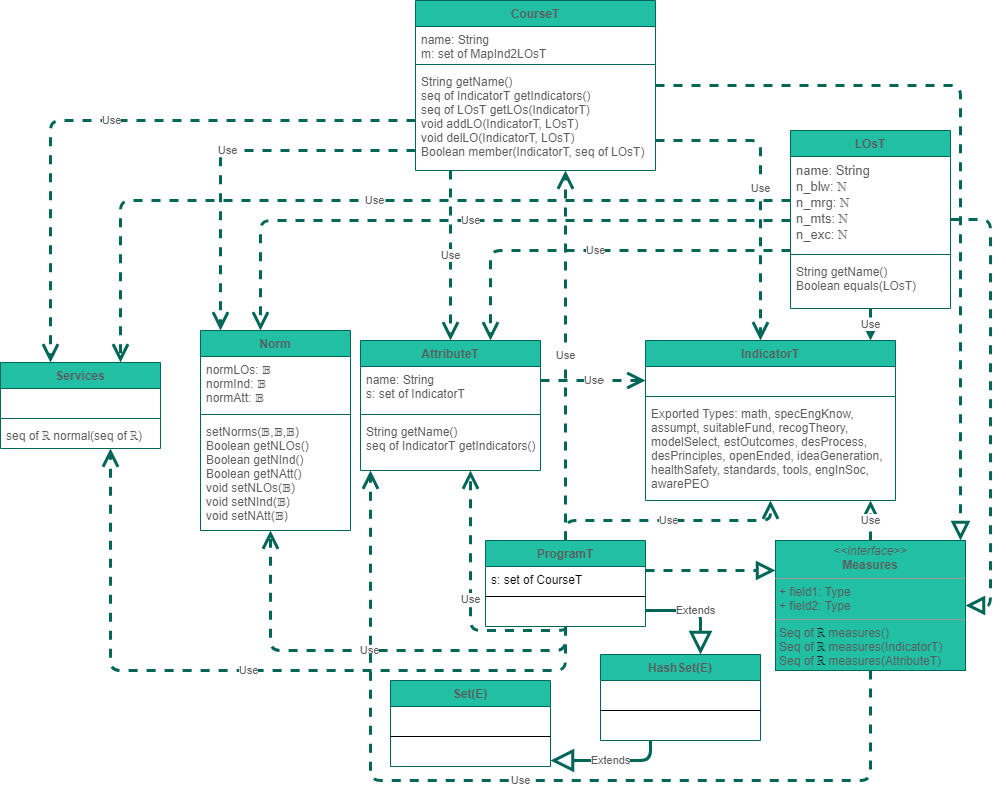
\includegraphics[width=1.2\textwidth]{UML.png} \\
  The UML is constructed using https://app.diagrams.net/
\end{center}

\medskip

\newpage

\noindent Q2: Draw a control flow graph for the convex hull algorithm.

\begin{center}
  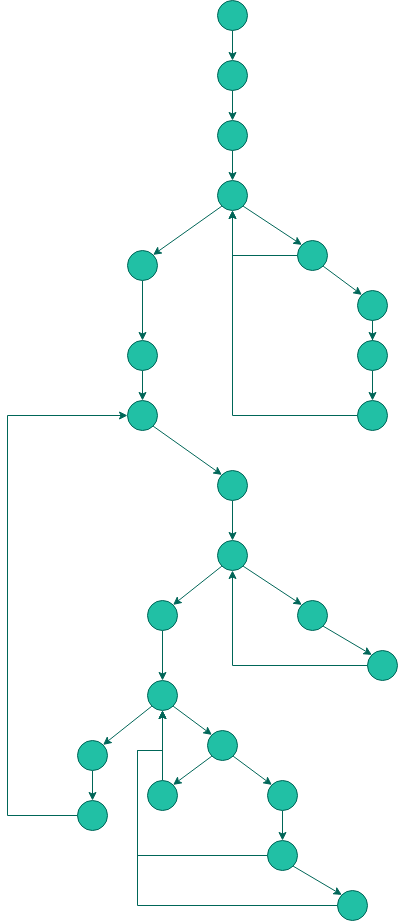
\includegraphics[width=0.5\textwidth]{Control_Flow_Graph.png} \\
  The control flow graph is constructed using https://app.diagrams.net/
\end{center}

\end {document}
